% !TeX program = xelatex
% ==========================================================================
% BAO CAO DO AN - CT603 KHAI PHA DU LIEU
% Dong tren day la "lenh ma thuat" bao Overleaf/TeXstudio tu dong bien dich
% bang XeLaTeX, khong can tu tay doi Compiler trong giao dien.
% ==========================================================================
\documentclass[12pt,a4paper]{report}

\usepackage{geometry}
\geometry{top=2.5cm,bottom=2.5cm,left=3cm,right=2cm}

\usepackage{fontspec}
\setmainfont{Times New Roman}

% Neu may ban khong co goi polyglossia-vietnamese, xoa/comment 2 dong duoi
% day di - tai lieu van bien dich binh thuong, chi mat phan ngat dong tieng Viet.
\usepackage{polyglossia}
\setmainlanguage{vietnamese}

\usepackage{graphicx}
\usepackage{booktabs}
\usepackage{array}
\usepackage{caption}
\usepackage{float}
\usepackage{enumitem}
\usepackage{setspace}
\onehalfspacing

\usepackage[hidelinks]{hyperref}

\graphicspath{{images/}}

% ----- Thong tin de tai -----
\newcommand{\tendetai}{Xây dựng mô hình dự đoán nguy cơ đột quỵ dựa trên các yếu tố lâm sàng và nhân khẩu học, so sánh hiệu quả giữa Decision Tree, k-NN và SVM}
\newcommand{\giangvien}{PGS.TS. Nguyễn Thái Nghe}
\newcommand{\sinhvienmot}{Lê Văn Triệu \hfill MSSV: M2526034}
\newcommand{\sinhvienhai}{La Quỳnh Như \hfill MSSV: M2526026}

\begin{document}

% ==========================================================================
% TRANG BIA
% ==========================================================================
\begin{titlepage}
\centering
\large
TRƯỜNG ĐẠI HỌC CẦN THƠ\\
TRƯỜNG CÔNG NGHỆ THÔNG TIN VÀ TRUYỀN THÔNG\\[2cm]

{\Large\bfseries BÁO CÁO ĐỀ TÀI}\\[0.5cm]
{\Large\bfseries MÔN KHO DỮ LIỆU VÀ KHAI PHÁ DỮ LIỆU (CTH603)}\\[1.5cm]

{\LARGE\bfseries \tendetai}\\[3cm]

\begin{minipage}{0.48\textwidth}
\centering
\textbf{Giảng viên hướng dẫn}\\[0.3cm]
\giangvien
\end{minipage}
\hfill
\begin{minipage}{0.48\textwidth}
\centering
\textbf{Sinh viên thực hiện}\\[0.3cm]
\sinhvienmot\\[0.2cm]
\sinhvienhai
\end{minipage}

\vfill
{\large Cần Thơ -- 2026}
\end{titlepage}

\tableofcontents
\clearpage

% ==========================================================================
% TOM TAT / ABSTRACT
% ==========================================================================
\chapter*{Tóm tắt}
\addcontentsline{toc}{chapter}{Tóm tắt}

Đột quỵ là một trong những nguyên nhân gây tử vong và tàn tật hàng đầu trên thế giới, trong khi việc phát hiện sớm nguy cơ có thể giúp can thiệp y tế kịp thời. Đồ án này xây dựng và so sánh ba mô hình máy học -- Decision Tree, k-Nearest Neighbors (k-NN) và Support Vector Machine (SVM) -- để dự đoán nguy cơ đột quỵ dựa trên các yếu tố lâm sàng và nhân khẩu học, sử dụng bộ dữ liệu Stroke Prediction Dataset (5.110 bệnh nhân, 12 thuộc tính) từ Kaggle. Do dữ liệu mất cân bằng lớp nặng (chỉ 4,87\% bệnh nhân có đột quỵ), đồ án tập trung xử lý vấn đề này bằng \texttt{class\_weight='balanced'} và điều chỉnh ngưỡng quyết định, đồng thời đánh giá bằng nhiều độ đo (Accuracy, Precision, Recall, F1, AUC, Confusion Matrix) thay vì chỉ dựa vào Accuracy. Sau khi dò tham số tối ưu cho từng mô hình và kiểm chứng bằng 5-fold Cross-Validation, kết quả cho thấy \textbf{SVM (kernel tuyến tính, C=0,01) đạt hiệu quả tốt nhất} với AUC = 0,8404 (một lần chia train/test) và AUC = 0,8379 $\pm$ 0,0249 (5-fold CV), vượt trội so với Decision Tree (AUC = 0,8305) và k-NN (AUC = 0,7831). Đồ án còn xây dựng một hệ thống demo đầy đủ (Backend Python/FastAPI, Frontend Next.js) cho phép người dùng nhập thông tin bệnh nhân để dự đoán, xem và tự điều chỉnh tham số mô hình, cũng như chạy lại trực tiếp quá trình dò tham số để kiểm chứng kết quả.

\textbf{Từ khóa:} dự đoán đột quỵ, Decision Tree, k-Nearest Neighbors, Support Vector Machine, mất cân bằng lớp, cross-validation.

\chapter*{Abstract}
\addcontentsline{toc}{chapter}{Abstract}

Stroke is one of the leading causes of death and disability worldwide, and early risk detection can enable timely medical intervention. This project builds and compares three machine learning models -- Decision Tree, k-Nearest Neighbors (k-NN), and Support Vector Machine (SVM) -- to predict stroke risk based on clinical and demographic factors, using the Stroke Prediction Dataset (5,110 patients, 12 attributes) from Kaggle. Given the severe class imbalance in the data (only 4.87\% of patients had a stroke), the project focuses on handling this issue via \texttt{class\_weight='balanced'} and decision-threshold tuning, and evaluates models using multiple metrics (Accuracy, Precision, Recall, F1, AUC, Confusion Matrix) rather than Accuracy alone. After hyperparameter tuning and verification via 5-fold Cross-Validation, results show that \textbf{SVM (linear kernel, C=0.01) performs best}, achieving AUC = 0.8404 (single train/test split) and AUC = 0.8379 $\pm$ 0.0249 (5-fold CV), outperforming Decision Tree (AUC = 0.8305) and k-NN (AUC = 0.7831). The project also delivers a full demo system (Python/FastAPI backend, Next.js frontend) that lets users enter patient information for prediction, view and adjust model parameters, and re-run the parameter search live to verify the results.

\textbf{Keywords:} stroke prediction, Decision Tree, k-Nearest Neighbors, Support Vector Machine, class imbalance, cross-validation.

\clearpage

% ==========================================================================
% CHUONG 1
% ==========================================================================
\chapter{Giới thiệu}

\section{Đặt vấn đề}

Theo Tổ chức Y tế Thế giới (WHO), đột quỵ là nguyên nhân gây tử vong đứng thứ hai trên toàn cầu và là nguyên nhân hàng đầu gây tàn tật lâu dài ở người trưởng thành. Việc phát hiện sớm các yếu tố nguy cơ -- như tuổi tác, tăng huyết áp, bệnh tim, mức glucose trong máu, chỉ số khối cơ thể (BMI), thói quen hút thuốc -- có ý nghĩa quan trọng trong việc hỗ trợ bác sĩ sàng lọc và tư vấn can thiệp kịp thời cho bệnh nhân có nguy cơ cao.

máy học (machine learning) là công cụ phù hợp để khai thác mối quan hệ giữa nhiều yếu tố lâm sàng/nhân khẩu học và nguy cơ đột quỵ, vốn khó mô hình hóa bằng các quy tắc thủ công đơn giản. Tuy nhiên, dữ liệu y tế thực tế thường gặp một thách thức lớn: \textbf{mất cân bằng lớp} -- số ca bệnh thực sự (dương tính) luôn chiếm tỉ lệ rất nhỏ so với số người khỏe mạnh. Nếu không xử lý đúng cách, mô hình có thể đạt độ chính xác (Accuracy) rất cao chỉ bằng cách luôn dự đoán "không có nguy cơ", trong khi trên thực tế lại không phát hiện được bất kỳ ca bệnh nào -- một vấn đề được gọi là "nghịch lý Accuracy" (Accuracy Paradox).

\section{Mục tiêu đề tài}

Đồ án đặt ra các mục tiêu sau:

\begin{enumerate}
    \item Xây dựng và huấn luyện ba mô hình phân lớp đã học trong môn Kho dữ liệu và khai phá dữ liệu -- Decision Tree, k-Nearest Neighbors (k-NN) và Support Vector Machine (SVM) -- trên bộ dữ liệu dự đoán đột quỵ.
    \item Dò tham số tối ưu cho từng mô hình (độ sâu cây, số K, ngưỡng quyết định, kernel và hệ số C) bằng thực nghiệm có bằng chứng số liệu cụ thể, không chọn tham số tùy tiện.
    \item Xử lý đúng đắn vấn đề mất cân bằng lớp và đánh giá mô hình bằng đầy đủ các độ đo phù hợp (Precision, Recall, F1, AUC/ROC, Confusion Matrix), không chỉ dựa vào Accuracy.
    \item So sánh khách quan 3 mô hình trên cùng một cách chia dữ liệu, rút ra kết luận mô hình nào phù hợp nhất cho bài toán này, và kiểm chứng lại bằng 5-fold Cross-Validation.
    \item Xây dựng một hệ thống demo hoàn chỉnh (giao diện web) cho phép nhập thông tin bệnh nhân và nhận kết quả dự đoán từ cả 3 mô hình, đồng thời minh chứng trực quan quá trình dò tham số đã thực hiện.
\end{enumerate}

\section{Phạm vi đề tài}

Đồ án sử dụng bộ dữ liệu công khai Stroke Prediction Dataset (Kaggle), không sử dụng dữ liệu bệnh viện thực tế do vấn đề bảo mật và quyền riêng tư. Ba mô hình được giới hạn trong phạm vi các thuật toán phân lớp đã học ở môn Kho dữ liệu và khai phá dữ liệu (Decision Tree, k-NN, SVM), không mở rộng sang các mô hình học sâu (deep learning). Hệ thống demo được xây dựng ở quy mô vừa đủ để minh họa và kiểm chứng kết quả nghiên cứu, không hướng tới triển khai thực tế trong môi trường bệnh viện.

% ==========================================================================
% CHUONG 2
% ==========================================================================
\chapter{Cơ sở lý thuyết}

\section{Decision Tree (Cây quyết định)}

Decision Tree là thuật toán phân lớp xây dựng một cấu trúc cây, trong đó mỗi nút trong biểu diễn một phép kiểm tra trên một thuộc tính (ví dụ: "tuổi $>$ 50?"), mỗi nhánh là kết quả của phép kiểm tra, và mỗi nút lá là một nhãn dự đoán. Cây được xây dựng bằng cách chọn thuộc tính phân chia tốt nhất tại mỗi bước dựa trên tiêu chí làm giảm độ hỗn tạp (impurity) của tập dữ liệu con, ví dụ chỉ số Gini hoặc Entropy. Ưu điểm của Decision Tree là dễ diễn giải (có thể đọc trực tiếp các luật quyết định), nhưng nhược điểm lớn là dễ \textbf{overfitting} (học quá khớp) nếu cây mọc quá sâu, khiến mô hình học theo nhiễu của từng điểm dữ liệu cụ thể thay vì quy luật tổng quát. Tham số quan trọng cần kiểm soát là \texttt{max\_depth} (độ sâu tối đa của cây).

\section{k-Nearest Neighbors (k-NN)}

k-NN là thuật toán phân lớp dựa trên khoảng cách: để dự đoán nhãn của một điểm dữ liệu mới, thuật toán tìm $K$ điểm dữ liệu "gần" nhất trong tập huấn luyện (theo một độ đo khoảng cách, thường là khoảng cách Euclid), rồi lấy nhãn chiếm đa số trong $K$ điểm đó làm kết quả dự đoán. k-NN không thực sự "học" một hàm tham số nào trong quá trình huấn luyện (gọi là thuật toán "lazy learning" -- chỉ ghi nhớ dữ liệu), mà toàn bộ việc tính toán diễn ra lúc dự đoán. Vì dựa trên khoảng cách, k-NN \textbf{nhạy cảm với thang đo của các thuộc tính} -- thuộc tính có khoảng giá trị lớn hơn sẽ chi phối khoảng cách tính toán nếu dữ liệu chưa được chuẩn hóa (ví dụ \texttt{avg\_glucose\_level} dao động 55--272 so với \texttt{hypertension} chỉ 0 hoặc 1) -- nên dữ liệu đầu vào cần được chuẩn hóa (StandardScaler) trước khi áp dụng.

\section{Support Vector Machine (SVM)}

SVM tìm một siêu phẳng (hyperplane) phân tách hai nhóm dữ liệu sao cho khoảng cách (margin) từ siêu phẳng đến các điểm dữ liệu gần nhất của mỗi nhóm (gọi là support vector) là lớn nhất. Khi dữ liệu không thể phân tách tuyến tính, SVM có thể dùng các hàm nhân (kernel) như \texttt{rbf} để ánh xạ dữ liệu sang không gian nhiều chiều hơn, nơi việc phân tách tuyến tính trở nên khả thi. Tham số \texttt{C} điều khiển mức độ "chấp nhận sai" trong lúc huấn luyện: \texttt{C} lớn ép mô hình phân loại đúng mọi điểm huấn luyện (dễ overfitting), \texttt{C} nhỏ cho phép một số điểm bị phân loại sai để đổi lấy một ranh giới tổng quát hơn. Giống Decision Tree, SVM hỗ trợ trực tiếp tham số \texttt{class\_weight} để xử lý mất cân bằng lớp ngay trong quá trình huấn luyện.

\section{Các độ đo đánh giá mô hình}

\begin{itemize}
    \item \textbf{Accuracy}: tỉ lệ dự đoán đúng trên tổng số mẫu. Không đáng tin cậy khi dữ liệu mất cân bằng lớp nặng.
    \item \textbf{Precision}: trong số các ca được dự đoán "có đột quỵ", bao nhiêu phần trăm thực sự đúng.
    \item \textbf{Recall}: trong số các ca thực sự "có đột quỵ", mô hình phát hiện đúng được bao nhiêu phần trăm -- độ đo quan trọng nhất trong bài toán y tế vì bỏ sót một ca bệnh thật (False Negative) nguy hiểm hơn nhiều so với báo động giả.
    \item \textbf{F1-score}: trung bình điều hòa (harmonic mean) giữa Precision và Recall, cân bằng cả hai.
    \item \textbf{AUC (Area Under the ROC Curve)}: đo khả năng \emph{xếp hạng} của mô hình (phân biệt ai có nguy cơ cao hơn ai) trên toàn bộ các ngưỡng quyết định có thể, không phụ thuộc vào một ngưỡng cụ thể. AUC = 0,5 tương đương đoán ngẫu nhiên, AUC = 1,0 là phân biệt hoàn hảo.
    \item \textbf{Confusion Matrix (ma trận nhầm lẫn)}: bảng 2$\times$2 thể hiện số lượng True Positive (TP), True Negative (TN), False Positive (FP), False Negative (FN) -- là cơ sở để tính mọi độ đo ở trên.
\end{itemize}

\section{Cross-Validation (Kiểm định chéo)}

Kiểm định chéo k-fold là kỹ thuật chia dữ liệu thành $k$ phần bằng nhau, lần lượt dùng $k-1$ phần để huấn luyện và 1 phần còn lại để kiểm tra, lặp lại $k$ lần sao cho mỗi phần đều được dùng để kiểm tra đúng một lần. Kết quả cuối cùng là trung bình và độ lệch chuẩn của các độ đo qua $k$ lần lặp. Mục đích chính là kiểm chứng rằng kết quả đánh giá mô hình không phải do may rủi của một cách chia dữ liệu cụ thể, mà ổn định qua nhiều cách chia khác nhau. Với dữ liệu mất cân bằng lớp, cần dùng \textbf{Stratified k-fold} thay vì k-fold thông thường, để đảm bảo mỗi phần đều giữ đúng tỉ lệ lớp dương tính, tránh trường hợp một phần không có ca bệnh nào.

% ==========================================================================
% CHUONG 3
% ==========================================================================
\chapter{Dữ liệu và phương pháp thực hiện}

\section{Bộ dữ liệu}

Đồ án sử dụng bộ dữ liệu \textbf{Stroke Prediction Dataset}, tác giả fedesoriano, công bố công khai trên Kaggle\footnote{\url{https://www.kaggle.com/datasets/fedesoriano/stroke-prediction-dataset}}. Tác giả ghi nguồn gốc dữ liệu là "Confidential Source" (không công bố bệnh viện/tổ chức cụ thể cung cấp) -- đây là bộ dữ liệu công khai phổ biến trong học thuật, không phải dữ liệu chính thống từ một cơ quan y tế cụ thể.

Bộ dữ liệu gồm \textbf{5.110 bệnh nhân} và \textbf{12 thuộc tính}, trình bày ở Bảng~\ref{tab:cotdulieu}.

\begin{table}[H]
\centering
\caption{Cấu trúc bộ dữ liệu}
\label{tab:cotdulieu}
\begin{tabular}{ll}
\toprule
\textbf{Thuộc tính} & \textbf{Ý nghĩa} \\
\midrule
id & Mã bệnh nhân (loại bỏ khi huấn luyện) \\
gender & Giới tính \\
age & Tuổi \\
hypertension & Tăng huyết áp (0/1) \\
heart\_disease & Bệnh tim (0/1) \\
ever\_married & Tình trạng hôn nhân \\
work\_type & Loại công việc \\
Residence\_type & Nơi ở (thành thị/nông thôn) \\
avg\_glucose\_level & Mức glucose trung bình trong máu \\
bmi & Chỉ số khối cơ thể (có giá trị thiếu) \\
smoking\_status & Tình trạng hút thuốc \\
\textbf{stroke} & \textbf{Nhãn mục tiêu} -- 1 = có đột quỵ, 0 = không \\
\bottomrule
\end{tabular}
\end{table}

\subsection{Thống kê mô tả}

Khảo sát thực tế trên dữ liệu cho thấy:
\begin{itemize}
    \item Cột \texttt{bmi} thiếu 201/5.110 giá trị (3,9\%).
    \item Nhãn \texttt{stroke} mất cân bằng lớp \textbf{rất nặng}: 4.861 người không đột quỵ (95,13\%) so với chỉ 249 người có đột quỵ (4,87\%).
    \item 5 thuộc tính dạng chữ (\texttt{gender}, \texttt{ever\_married}, \texttt{work\_type}, \texttt{Residence\_type}, \texttt{smoking\_status}) cần được mã hóa thành số trước khi đưa vào mô hình.
\end{itemize}

Đây chính là lý do đồ án phải báo cáo đầy đủ Precision/Recall/F1/AUC thay vì chỉ Accuracy: một mô hình luôn dự đoán "không đột quỵ" vẫn đạt Accuracy $\approx$ 95\% nhưng hoàn toàn vô dụng về mặt y khoa.

\subsection{Tiền xử lý dữ liệu}

Các bước tiền xử lý được thực hiện gồm:
\begin{enumerate}
    \item \textbf{Điền giá trị thiếu}: 201 ô trống ở cột \texttt{bmi} được điền bằng giá trị trung vị (median = 28,1) thay vì trung bình, vì trung vị ít bị ảnh hưởng bởi các giá trị BMI bất thường, phù hợp hơn với dữ liệu y tế vốn dễ có ngoại lệ.
    \item \textbf{Loại bỏ cột} \texttt{id}: chỉ là mã định danh, không mang thông tin y khoa, có thể khiến mô hình học sai lệch theo thứ tự.
    \item \textbf{Mã hóa biến phân loại} (Label Encoding) cho 5 cột dạng chữ -- chuyển mỗi giá trị chữ thành một số nguyên tương ứng (ví dụ \texttt{gender}: Male=0, Female=1, Other=2). Các con số này chỉ mang tính ký hiệu phân loại, không thể hiện thứ tự hơn kém.
\end{enumerate}

Sau tiền xử lý, dữ liệu còn 5.110 dòng, 11 cột, không còn ô trống hay cột dạng chữ, sẵn sàng đưa vào huấn luyện.

\section{Phương pháp chia dữ liệu}

Toàn bộ 3 mô hình được huấn luyện và đánh giá trên \textbf{cùng một cách chia dữ liệu} để đảm bảo so sánh công bằng: 80\% huấn luyện (4.088 dòng) / 20\% kiểm tra (1.022 dòng), dùng \texttt{train\_test\_split(..., test\_size=0.2, random\_state=42, stratify=y)}. Tham số \texttt{stratify=y} đảm bảo tỉ lệ nhãn \texttt{stroke=1} ($\approx$ 4,87--4,89\%) được giữ đều ở cả tập huấn luyện và tập kiểm tra, tránh trường hợp tập kiểm tra ngẫu nhiên có quá ít hoặc quá nhiều ca đột quỵ.

\section{Phương pháp dò tham số và xử lý mất cân bằng lớp}

Mỗi mô hình được dò nhiều giá trị tham số khác nhau trên cùng tập dữ liệu, chọn cấu hình tốt nhất theo tiêu chí AUC cao nhất (phù hợp với dữ liệu mất cân bằng, không phụ thuộc một ngưỡng cụ thể):

\begin{itemize}
    \item \textbf{Decision Tree}: dò \texttt{max\_depth} từ 1 đến 20 (và không giới hạn), kết hợp \texttt{class\_weight='balanced'}.
    \item \textbf{k-NN}: dò $K$ từ 1 đến 30, với 2 cách tính trọng số hàng xóm (\texttt{uniform}, \texttt{distance}), trên dữ liệu đã chuẩn hóa; sau đó dò thêm ngưỡng quyết định (decision threshold) vì k-NN không hỗ trợ \texttt{class\_weight}.
    \item \textbf{SVM}: dò \texttt{kernel} (\texttt{linear}, \texttt{rbf}) $\times$ \texttt{C} (0,01 đến 10), kết hợp \texttt{class\_weight='balanced'}, trên dữ liệu đã chuẩn hóa.
\end{itemize}

Decision Tree và SVM xử lý mất cân bằng lớp trực tiếp qua \texttt{class\_weight='balanced'} (tác động vào hàm mục tiêu lúc huấn luyện). k-NN không có cơ chế tương tự (vì đây là thuật toán "ghi nhớ" dữ liệu, không học tham số), nên được bù lại bằng cách \textbf{hạ ngưỡng quyết định} sau khi huấn luyện, nhằm đạt mức Recall tương đương hai mô hình còn lại để so sánh công bằng.

\section{Phương pháp đánh giá cuối cùng}

Sau khi chốt cấu hình tốt nhất cho từng mô hình, đồ án thực hiện hai lớp kiểm chứng:
\begin{enumerate}
    \item \textbf{So sánh trên 1 lần chia train/test}: huấn luyện lại cả 3 mô hình với cấu hình đã chốt trên cùng một tập train/test, tính đầy đủ Accuracy, Precision, Recall, F1, AUC, Confusion Matrix, vẽ đường cong ROC.
    \item \textbf{5-fold Stratified Cross-Validation}: chạy lại đúng cấu hình tốt nhất của mỗi mô hình qua 5 lần chia dữ liệu khác nhau, tính trung bình và độ lệch chuẩn của AUC/Recall -- để xác nhận kết quả ở bước (1) không phải do may rủi của một cách chia dữ liệu cụ thể.
\end{enumerate}

% ==========================================================================
% CHUONG 4
% ==========================================================================
\chapter{Kết quả thực nghiệm và xây dựng hệ thống demo}

\section{Kết quả dò tham số từng mô hình}

\subsection{Decision Tree}

Phiên bản Decision Tree mặc định (không giới hạn độ sâu) cho thấy dấu hiệu overfitting rõ rệt: Accuracy trên tập huấn luyện đạt 100\% trong khi trên tập kiểm tra chỉ 91,68\%, với cây mọc sâu tới 18 tầng và 289 lá. Sau khi dò \texttt{max\_depth} từ 1 đến 20, cấu hình tốt nhất được chọn là \texttt{max\_depth=4, class\_weight='balanced'}, đạt AUC = 0,8305 (Hình~\ref{fig:dtchart}).

\subsection{k-Nearest Neighbors}

Thử nghiệm ban đầu với $K=5$ cho thấy Recall gần như bằng 0, do với chỉ $\approx$5\% dữ liệu thuộc nhóm dương tính, xác suất tìm đủ đa số hàng xóm thuộc nhóm này rất thấp. Sau khi dò $K$ từ 1 đến 30, cấu hình $K=16$, \texttt{weights='uniform'} đạt AUC cao nhất = 0,7831, nhưng Recall vẫn bằng 0 ở ngưỡng mặc định 0,5 (AUC đo khả năng xếp hạng, không đo quyết định ở một ngưỡng cụ thể). Dò thêm ngưỡng quyết định, ngưỡng \textbf{0,06} được chọn để đạt Recall = 84\%, tương đương Decision Tree, phục vụ so sánh công bằng.

\subsection{Support Vector Machine}

Dò 12 cấu hình (\texttt{kernel} $\times$ \texttt{C}), cấu hình tốt nhất là \texttt{kernel='linear', C=0,01, class\_weight='balanced'}, đạt AUC = \textbf{0,8404} -- cao nhất trong cả 3 mô hình -- và đạt Recall = 84\% ngay ở ngưỡng mặc định, không cần kỹ thuật hạ ngưỡng như k-NN.

\begin{table}[H]
\centering
\caption{Cấu hình tốt nhất của từng mô hình}
\label{tab:cauhinh}
\begin{tabular}{lll}
\toprule
\textbf{Mô hình} & \textbf{Tham số tốt nhất} & \textbf{AUC} \\
\midrule
Decision Tree & max\_depth=4, class\_weight='balanced' & 0,8305 \\
k-NN & K=16, weights='uniform', threshold=0,06 & 0,7831 \\
\textbf{SVM} & \textbf{kernel='linear', C=0,01, class\_weight='balanced'} & \textbf{0,8404} \\
\bottomrule
\end{tabular}
\end{table}

\section{So sánh tổng hợp và kết luận chính}

Huấn luyện lại cả 3 mô hình với cấu hình đã chốt trên cùng tập train/test, canh cùng mức Recall = 84\% (cùng bắt đúng 42/50 ca đột quỵ thật trong tập kiểm tra, bỏ sót 8/50 ca) để so sánh công bằng tuyệt đối (Bảng~\ref{tab:sosanh}).

\begin{table}[H]
\centering
\caption{So sánh tổng hợp 3 mô hình (cùng mức Recall = 0,84)}
\label{tab:sosanh}
\begin{tabular}{lccccc}
\toprule
\textbf{Mô hình} & \textbf{Accuracy} & \textbf{Precision} & \textbf{Recall} & \textbf{F1} & \textbf{AUC} \\
\midrule
\textbf{SVM} & \textbf{0,7260} & \textbf{0,1338} & 0,84 & \textbf{0,2308} & \textbf{0,8404} \\
Decision Tree & 0,6526 & 0,1080 & 0,84 & 0,1913 & 0,8305 \\
k-NN & 0,6370 & 0,1037 & 0,84 & 0,1846 & 0,7831 \\
\bottomrule
\end{tabular}
\end{table}

Ở cùng mức Recall, \textbf{SVM thắng ở cả 4/4 độ đo còn lại}. Ba lý do giải thích kết quả này:
\begin{enumerate}
    \item \texttt{class\_weight='balanced'} của SVM tác động trực tiếp vào hàm mục tiêu khi huấn luyện, giống Decision Tree -- trong khi k-NN phải dùng kỹ thuật "hạ ngưỡng sau khi huấn luyện", vốn kém tối ưu hơn.
    \item Ranh giới phân tách 2 nhóm trong dữ liệu khá đơn giản (\texttt{kernel='linear'} thắng \texttt{'rbf'} ở mọi giá trị C), phù hợp với cách SVM tìm một siêu phẳng tối ưu toàn cục -- trong khi k-NN chỉ dựa vào các điểm lân cận cục bộ, dễ bị nhiễu.
    \item Tham số \texttt{C} nhỏ (mô hình "mềm dẻo") tổng quát hóa tốt hơn, nhất quán với bài học tránh overfitting rút ra từ Decision Tree.
\end{enumerate}

\textbf{Kết luận chính thức:} Trong 3 mô hình đã thử nghiệm trên bộ dữ liệu Stroke Prediction, \textbf{SVM với kernel tuyến tính, C=0,01, class\_weight='balanced' là mô hình tối ưu nhất}, cân bằng tốt nhất giữa khả năng phát hiện đúng ca có nguy cơ đột quỵ và độ chính xác tổng thể.

\section{Kiểm chứng bằng 5-fold Cross-Validation}

Để xác nhận kết quả trên không phải do may rủi của một cách chia dữ liệu, đồ án chạy bổ sung 5-fold Stratified Cross-Validation cho cấu hình tốt nhất của cả 3 mô hình (Bảng~\ref{tab:cv}).

\begin{table}[H]
\centering
\caption{Kết quả 5-fold Cross-Validation (trung bình $\pm$ độ lệch chuẩn qua 5 fold)}
\label{tab:cv}
\begin{tabular}{lcc}
\toprule
\textbf{Mô hình} & \textbf{AUC (CV)} & \textbf{Recall (CV)} \\
\midrule
Decision Tree & 0,7853 $\pm$ 0,0239 & 0,6985 $\pm$ 0,0929 \\
k-NN & 0,7098 $\pm$ 0,0200 & 0,7551 $\pm$ 0,0251 \\
\textbf{SVM} & \textbf{0,8379 $\pm$ 0,0249} & 0,8069 $\pm$ 0,0564 \\
\bottomrule
\end{tabular}
\end{table}

Kết quả cho thấy \textbf{thứ hạng 3 mô hình không đổi} (SVM $>$ Decision Tree $>$ k-NN) giữa 2 cách đánh giá, với độ lệch chuẩn AUC nhỏ (0,02--0,025) -- xác nhận kết quả ổn định, không phải ngẫu nhiên, củng cố thêm độ tin cậy cho kết luận chính của đồ án.

\section{Xây dựng hệ thống demo}

\subsection{Kiến trúc hệ thống}

Hệ thống demo được xây dựng theo kiến trúc client--server, tách biệt phần xử lý mô hình (Backend) và phần giao diện (Frontend):

\begin{itemize}
    \item \textbf{Backend -- Python (scikit-learn, FastAPI)}: tiền xử lý dữ liệu, huấn luyện 3 mô hình, đóng gói thành các file \texttt{.pkl} (dùng thư viện \texttt{joblib}), và cung cấp API REST nhận thông tin bệnh nhân, trả về kết quả dự đoán của cả 3 mô hình.
    \item \textbf{Frontend -- Next.js (React, TypeScript)}: giao diện web, gọi API Backend, hiển thị kết quả và biểu đồ minh chứng.
\end{itemize}

Luồng dữ liệu tổng thể: \emph{Next.js (form nhập liệu) $\rightarrow$ gọi API FastAPI (chạy model đã train sẵn) $\rightarrow$ trả JSON kết quả 3 mô hình $\rightarrow$ Next.js hiển thị kết quả}.

\subsection{Các chức năng của hệ thống demo}

Hệ thống gồm 4 trang chức năng, trình bày lần lượt dưới đây.

\paragraph{Trang Thông tin đồ án.} Trang giới thiệu tổng quan, gồm 3 mục: thông tin đề tài/dữ liệu/mô hình (Hình~\ref{fig:thongtin}), danh sách chức năng của hệ thống (Hình~\ref{fig:chucnang}), và mô tả kỹ thuật (Hình~\ref{fig:kythuat}).

\begin{figure}[H]
\centering
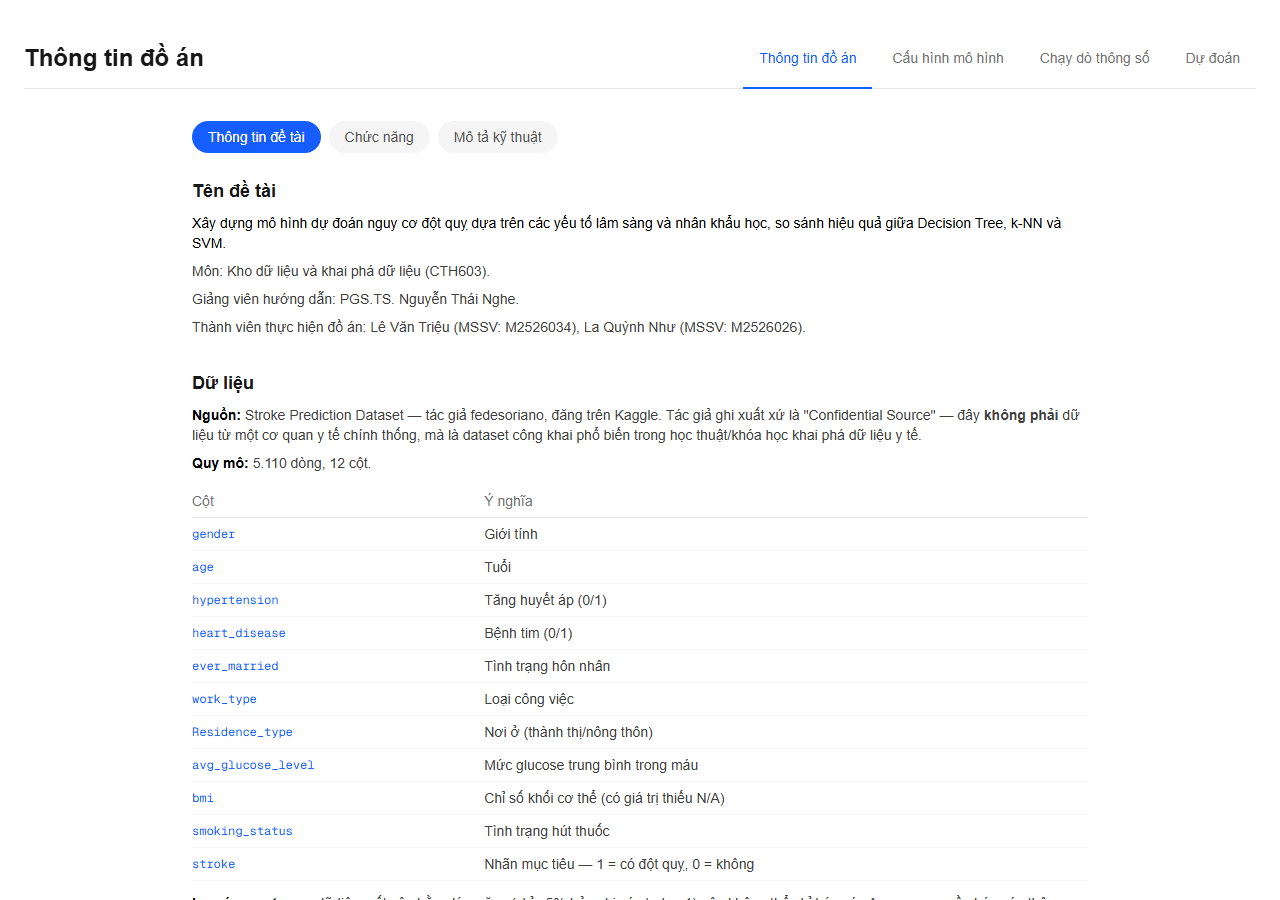
\includegraphics[width=0.95\textwidth]{01_thongtin_detai.png}
\caption{Trang Thông tin đồ án -- mục Thông tin đề tài}
\label{fig:thongtin}
\end{figure}

\begin{figure}[H]
\centering
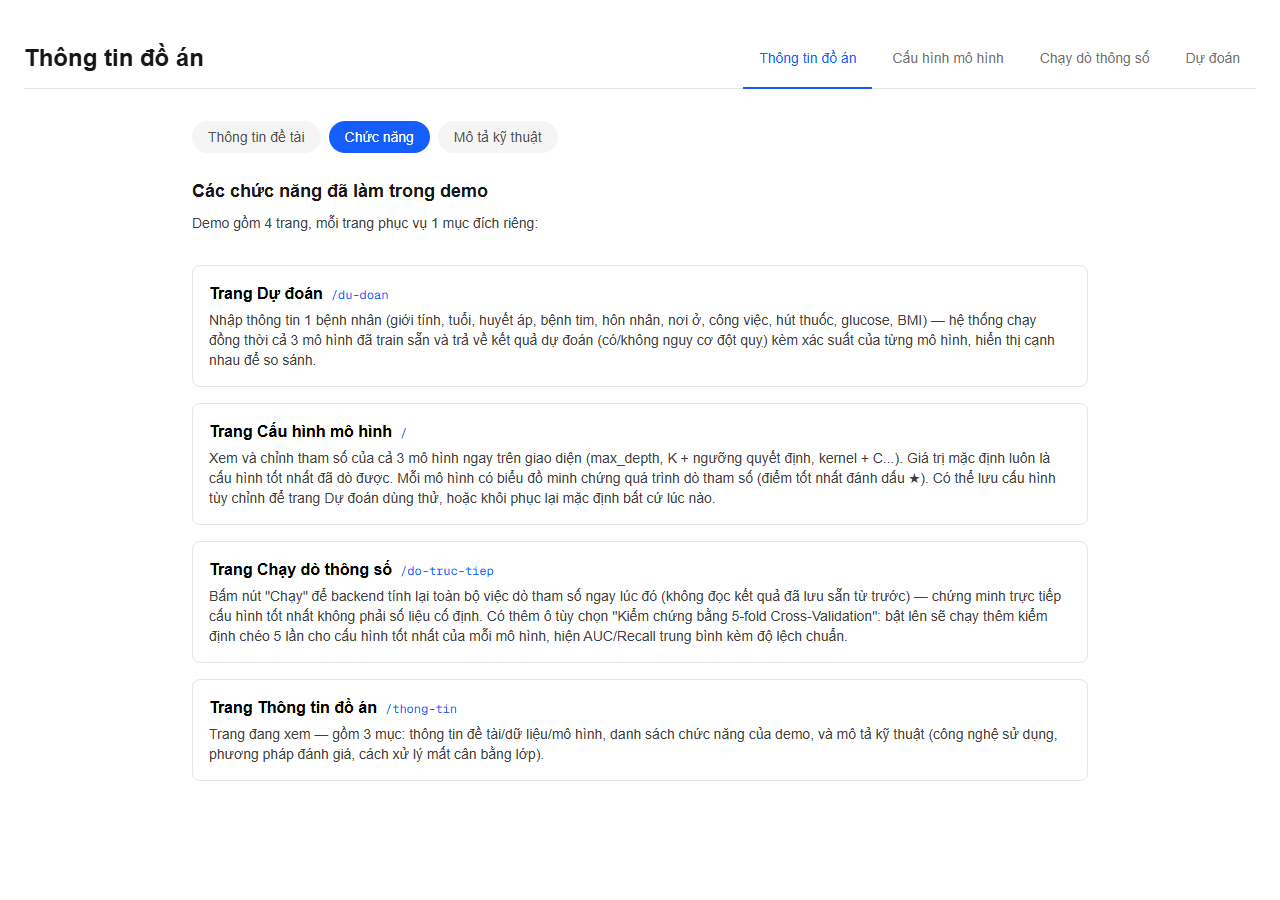
\includegraphics[width=0.95\textwidth]{02_thongtin_chucnang.png}
\caption{Trang Thông tin đồ án -- mục Chức năng}
\label{fig:chucnang}
\end{figure}

\begin{figure}[H]
\centering
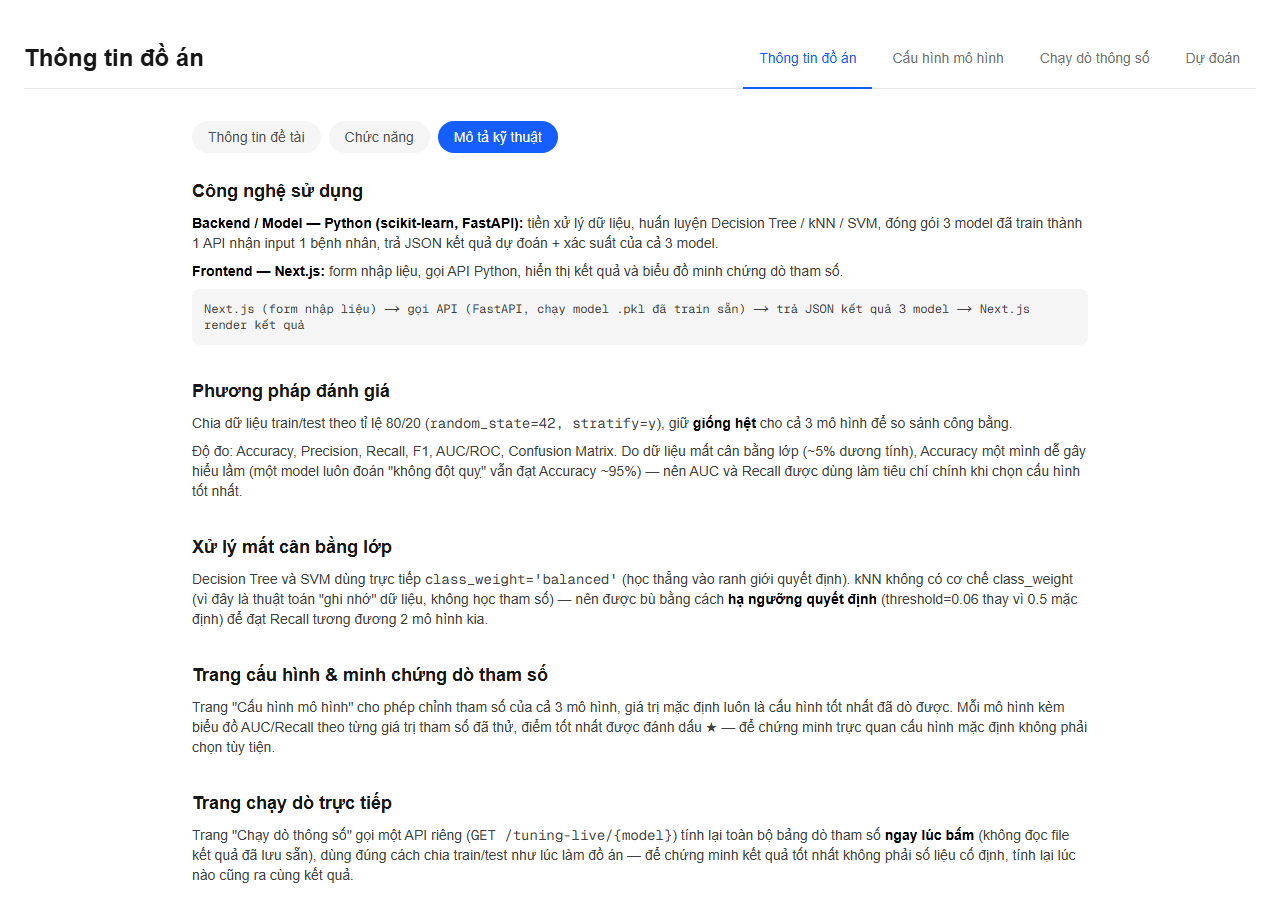
\includegraphics[width=0.95\textwidth]{03_thongtin_kythuat.png}
\caption{Trang Thông tin đồ án -- mục Mô tả kỹ thuật}
\label{fig:kythuat}
\end{figure}

\paragraph{Trang Cấu hình mô hình.} Cho phép người dùng xem và điều chỉnh tham số của cả 3 mô hình trực tiếp trên giao diện. Giá trị mặc định luôn là cấu hình tốt nhất đã dò được. Mỗi mô hình kèm biểu đồ AUC/Recall theo từng giá trị tham số đã thử, điểm tốt nhất được đánh dấu sao ($\bigstar$) -- để chứng minh trực quan rằng cấu hình mặc định không phải chọn tùy tiện mà có thực nghiệm đứng sau (Hình~\ref{fig:cauhinh}).

\begin{figure}[H]
\centering
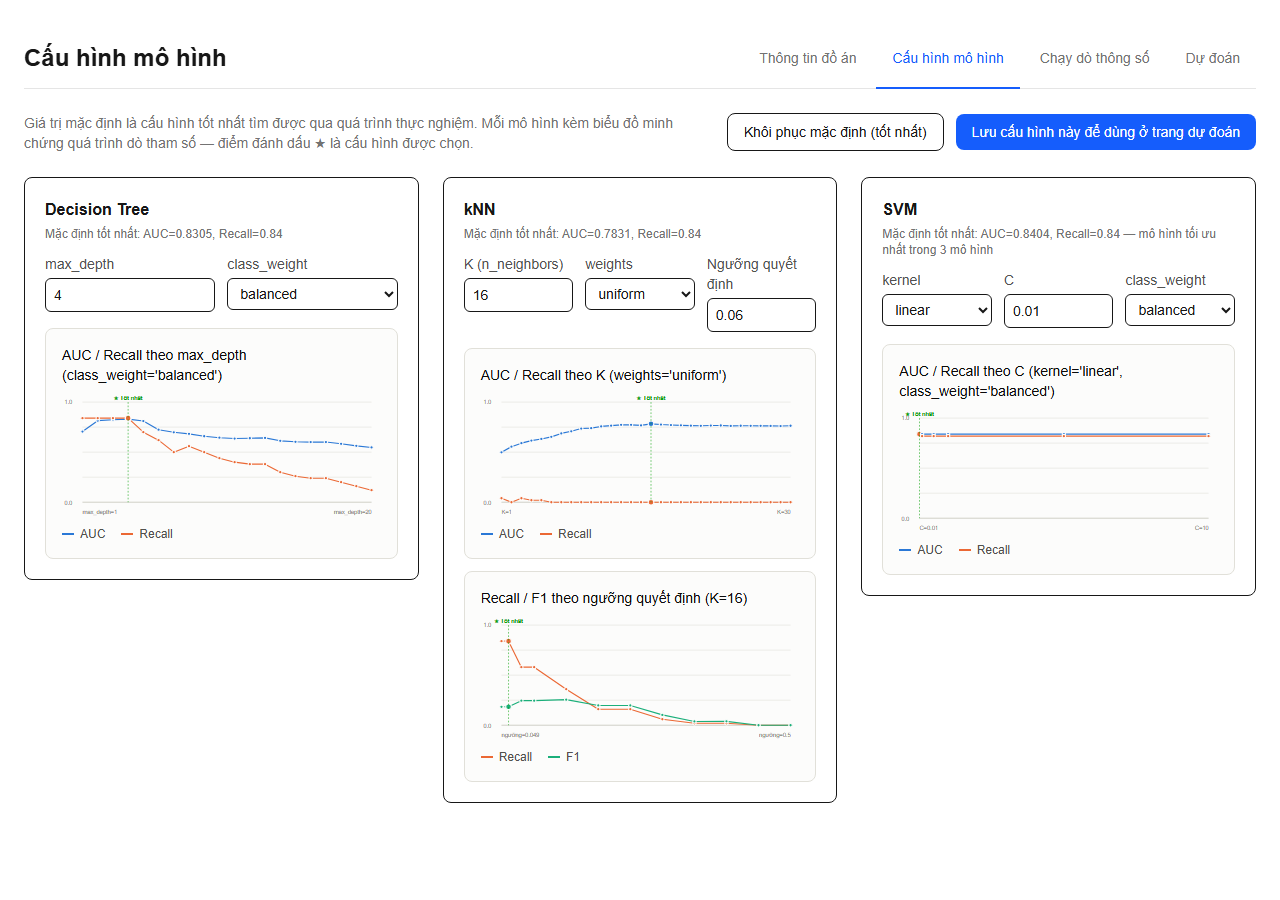
\includegraphics[width=0.95\textwidth]{04_cauhinh_mohinh.png}
\caption{Trang Cấu hình mô hình, kèm biểu đồ minh chứng dò tham số}
\label{fig:cauhinh}
\end{figure}

\paragraph{Trang Dự đoán.} Người dùng nhập thông tin một bệnh nhân (giới tính, tuổi, huyết áp, bệnh tim, hôn nhân, nơi ở, công việc, hút thuốc, glucose, BMI) (Hình~\ref{fig:dudoanform}); hệ thống chạy đồng thời cả 3 mô hình và trả về kết quả dự đoán kèm xác suất của từng mô hình để so sánh (Hình~\ref{fig:dudoanketqua}).

\begin{figure}[H]
\centering
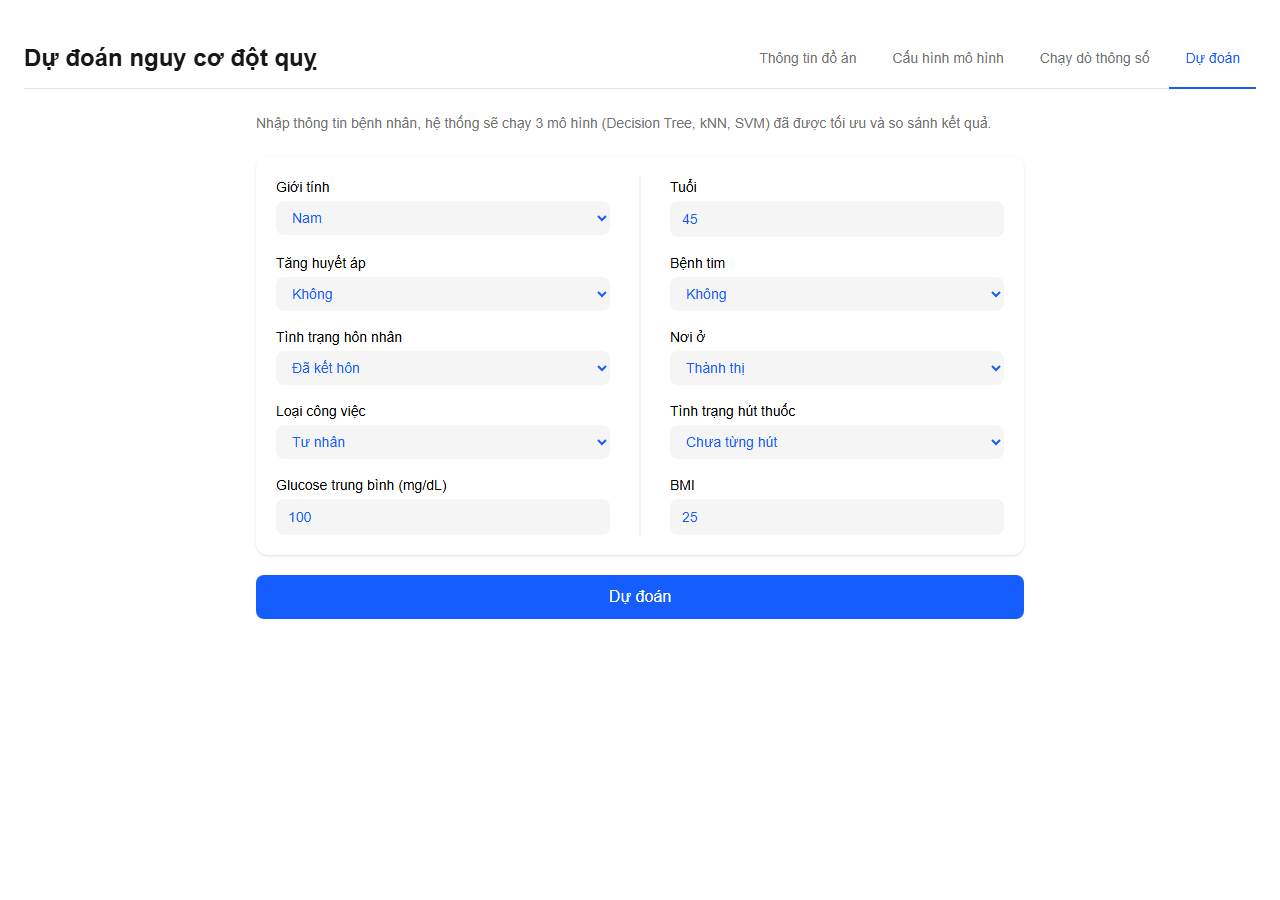
\includegraphics[width=0.75\textwidth]{05_dudoan_form.png}
\caption{Trang Dự đoán -- biểu mẫu nhập thông tin bệnh nhân}
\label{fig:dudoanform}
\end{figure}

\begin{figure}[H]
\centering
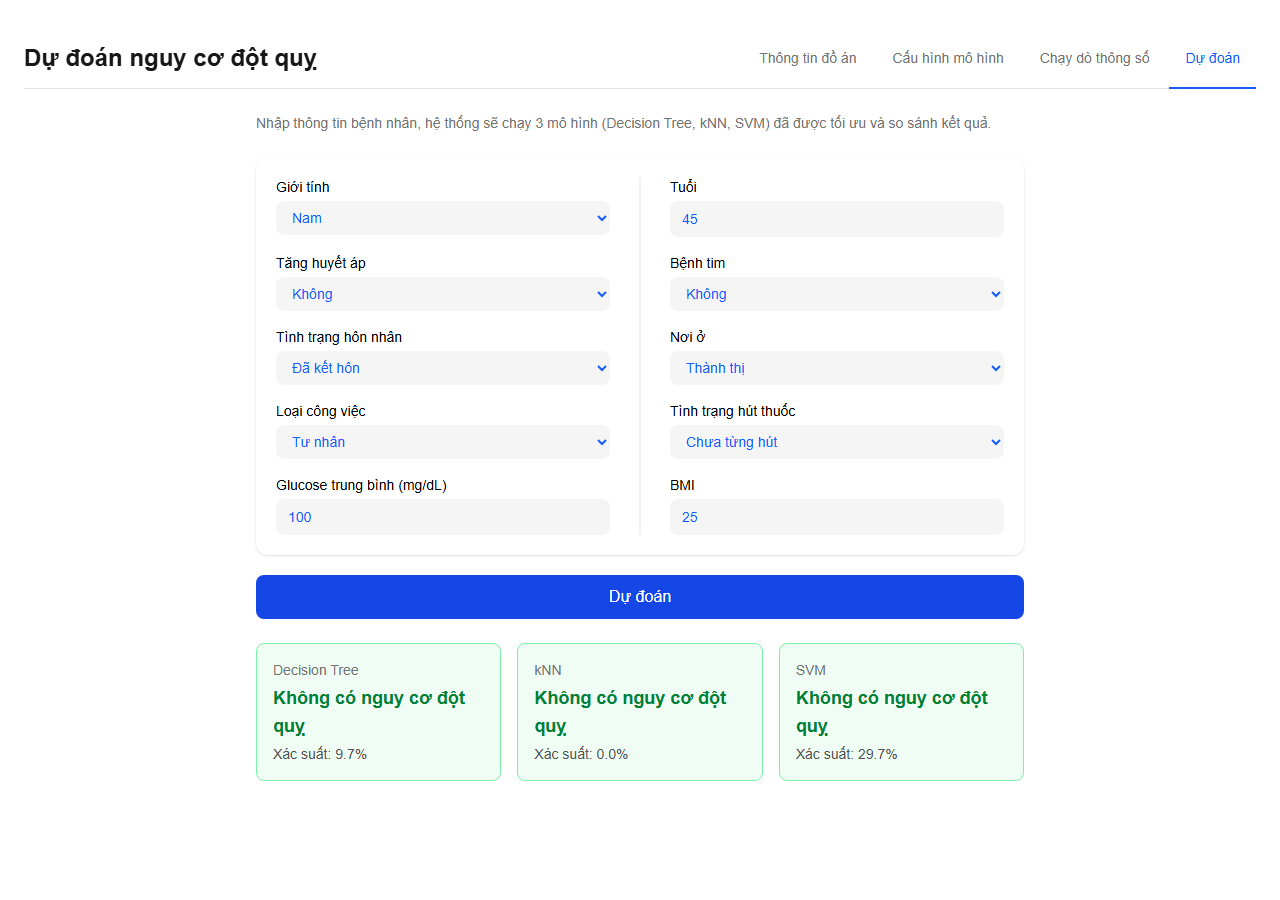
\includegraphics[width=0.75\textwidth]{06_dudoan_ketqua.png}
\caption{Trang Dự đoán -- kết quả dự đoán từ cả 3 mô hình}
\label{fig:dudoanketqua}
\end{figure}

\paragraph{Trang Chạy dò thông số.} Điểm đặc biệt của hệ thống: khi bấm nút "Chạy", Backend \textbf{tính lại toàn bộ việc dò tham số ngay lúc đó} (không đọc kết quả đã lưu sẵn từ trước), cùng cách chia dữ liệu như lúc làm đồ án -- chứng minh trực tiếp rằng cấu hình tốt nhất không phải số liệu cố định (Hình~\ref{fig:dothamsotruoc}). Trang này còn có tùy chọn "Kiểm chứng bằng 5-fold Cross-Validation": khi bật, hệ thống chạy thêm kiểm định chéo 5 lần cho cấu hình tốt nhất của mỗi mô hình và hiển thị kết quả (Hình~\ref{fig:dothamsoketqua}).

\begin{figure}[H]
\centering
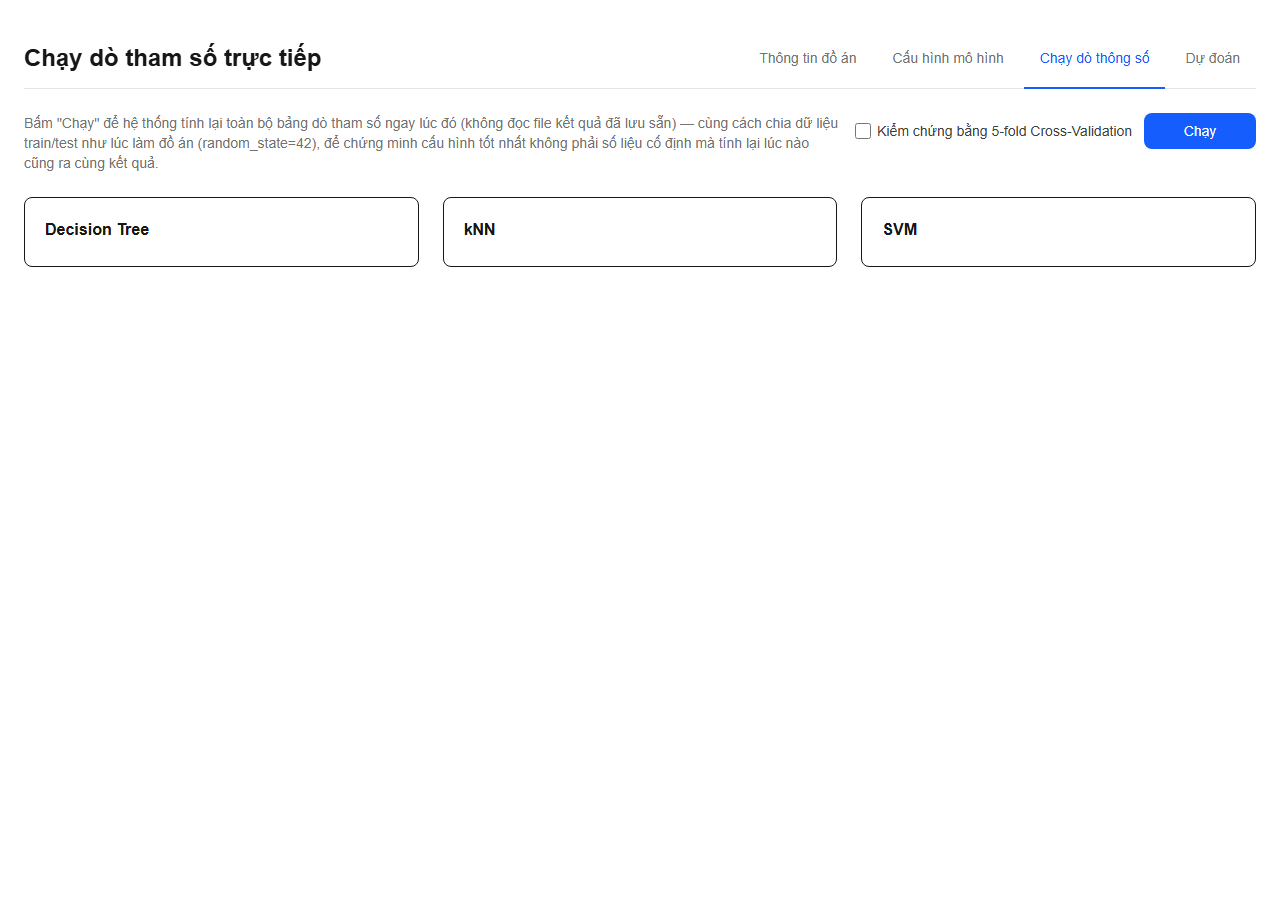
\includegraphics[width=0.75\textwidth]{07_dothamso_truockhi.png}
\caption{Trang Chạy dò thông số -- trước khi bấm chạy}
\label{fig:dothamsotruoc}
\end{figure}

\begin{figure}[H]
\centering
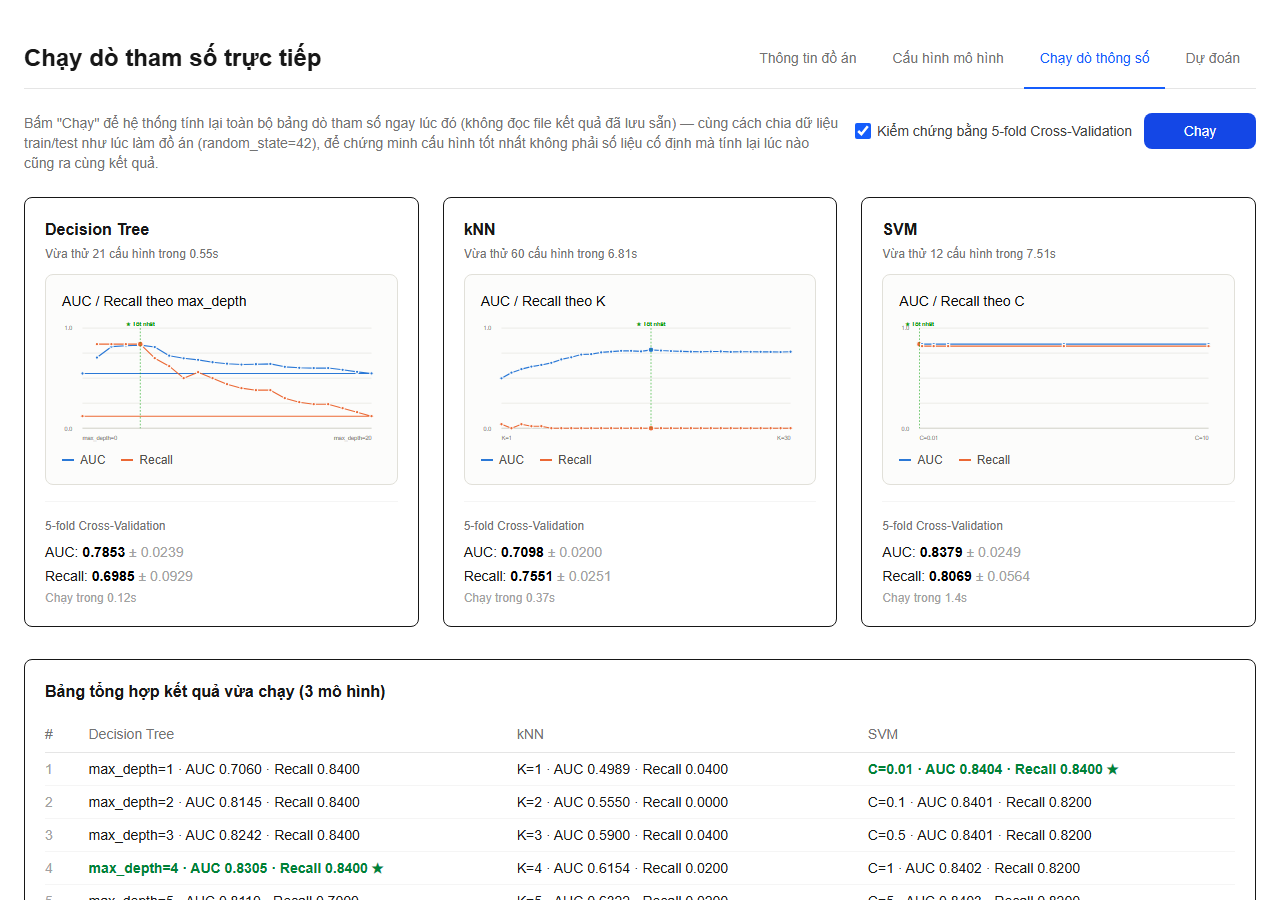
\includegraphics[width=0.95\textwidth]{08_dothamso_ketqua.png}
\caption{Trang Chạy dò thông số -- kết quả sau khi chạy, kèm kiểm chứng 5-fold Cross-Validation}
\label{fig:dothamsoketqua}
\end{figure}

% ==========================================================================
% CHUONG 5
% ==========================================================================
\chapter{Kết luận và hướng phát triển}

\section{Kết luận}

Đồ án đã hoàn thành đầy đủ các mục tiêu đề ra: xây dựng và dò tham số tối ưu cho 3 mô hình Decision Tree, k-NN và SVM trên bộ dữ liệu dự đoán đột quỵ; xử lý đúng đắn vấn đề mất cân bằng lớp bằng \texttt{class\_weight='balanced'} và điều chỉnh ngưỡng quyết định; đánh giá khách quan bằng nhiều độ đo phù hợp (Precision, Recall, F1, AUC, Confusion Matrix) thay vì chỉ Accuracy; và kiểm chứng kết quả bằng 5-fold Cross-Validation.

Kết quả thực nghiệm khẳng định \textbf{SVM với kernel tuyến tính, C=0,01, class\_weight='balanced'} là mô hình phù hợp nhất cho bài toán này, đạt AUC = 0,8404 (một lần chia train/test) và AUC = 0,8379 $\pm$ 0,0249 (5-fold Cross-Validation), vượt trội và ổn định hơn Decision Tree và k-NN. Đồ án cũng xây dựng thành công một hệ thống demo đầy đủ chức năng, cho phép người dùng (kể cả không chuyên về kỹ thuật) tương tác trực tiếp với cả 3 mô hình, tự điều chỉnh tham số, và quan trọng nhất là \textbf{tự kiểm chứng lại} quá trình dò tham số và kiểm định chéo bất cứ lúc nào, thay vì chỉ xem số liệu tĩnh.

\section{Hạn chế}

\begin{itemize}
    \item Bộ dữ liệu sử dụng là dữ liệu công khai từ Kaggle, nguồn gốc không được công bố rõ ràng (ghi "Confidential Source"), nên kết quả mang tính minh họa phương pháp luận, chưa thể khẳng định độ chính xác lâm sàng trên dữ liệu bệnh viện thực tế.
    \item Do dữ liệu mất cân bằng lớp nặng, cả 3 mô hình đều có Precision thấp (10--13\%) ở mức Recall 84\% -- nghĩa là có nhiều "báo động giả", cần cân nhắc thêm khi ứng dụng thực tế.
    \item Đồ án giới hạn trong 3 mô hình đã học ở môn học, chưa thử nghiệm các kỹ thuật cân bằng dữ liệu khác (như SMOTE) hay các mô hình phức tạp hơn (ensemble, deep learning).
\end{itemize}

\section{Hướng phát triển}

\begin{itemize}
    \item Thử nghiệm thêm các kỹ thuật xử lý mất cân bằng lớp khác (SMOTE, undersampling) và so sánh với cách tiếp cận \texttt{class\_weight} hiện tại.
    \item Mở rộng so sánh với các mô hình máy học khác (Random Forest, Gradient Boosting, mạng nơ-ron) để có cái nhìn toàn diện hơn.
    \item Nếu có điều kiện tiếp cận dữ liệu bệnh viện thực tế (có kiểm soát quyền riêng tư đúng quy định), kiểm chứng lại mô hình trên dữ liệu đó để đánh giá khả năng ứng dụng thực tiễn.
    \item Hoàn thiện hệ thống demo thành công cụ sàng lọc hỗ trợ bác sĩ, bổ sung xác thực người dùng và lưu trữ lịch sử dự đoán.
\end{itemize}

% ==========================================================================
% TAI LIEU THAM KHAO
% ==========================================================================
\begin{thebibliography}{9}

\bibitem{dataset}
fedesoriano, \emph{Stroke Prediction Dataset}, Kaggle, 2021.
\url{https://www.kaggle.com/datasets/fedesoriano/stroke-prediction-dataset}

\bibitem{sklearn}
Pedregosa, F. et al., \emph{Scikit-learn: Machine Learning in Python}, Journal of Machine Learning Research, 12, 2825--2830, 2011.

\bibitem{who}
World Health Organization, \emph{The top 10 causes of death}, WHO Fact Sheets, 2020.

\end{thebibliography}

\end{document}
